\chapter{FUNDAMENTOS} \label{chap:fundamentos}

El desarrollo de sistemas automatizados para la detección y clasificación de retinopatía
diabética mediante técnicas de aprendizaje profundo requiere una comprensión sólida de
múltiples dominios del conocimiento. Este capítulo presenta los fundamentos teóricos que
sustentan el presente trabajo, organizados en tres componentes principales: primero, se
describe la naturaleza y características de las imágenes de fondo de ojo, el principal
insumo del sistema propuesto; segundo, se expone la fisiopatología y clasificación
clínica de la retinopatía diabética; y tercero, se desarrollan los conceptos
fundamentales de inteligencia artificial, aprendizaje automático y redes neuronales
convolucionales que constituyen la base metodológica del trabajo.


\section{IMÁGENES DEL FONDO DE OJO}

Las imágenes de fondo de ojo, también conocidas como retinografías o imágenes de retina,
son fotografías detalladas de la parte posterior del ojo que permiten observar
estructuras clave como la retina, el nervio óptico, los vasos sanguíneos y la mácula.
Estas imágenes son fundamentales en oftalmología para el diagnóstico y seguimiento de
diversas enfermedades oculares, como la retinopatía diabética, el glaucoma, la
degeneración macular y otros trastornos retinianos. A través del análisis de estas
imágenes, los médicos pueden detectar alteraciones en los vasos sanguíneos, signos de
inflamación o daño estructural en la retina, lo que puede ser indicativo de enfermedades
en progresión.

El proceso de captura de estas imágenes se realiza mediante un examen médico no invasivo,
en el cual se emplea un oftalmoscopio o una cámara de fondo de ojo especializada. Este
instrumento emite una luz que atraviesa las pupilas y permite al especialista examinar
directamente la retina, los vasos sanguíneos y el nervio óptico. En la mayoría de los
casos, se requiere la dilatación de las pupilas para mejorar la visualización,
especialmente si se utiliza una cámara de fondo de ojo avanzada. Aunque la captura de
estas imágenes no es dolorosa, puede llevar algunos minutos, dependiendo de la tecnología
utilizada.

Existen varias técnicas para realizar la oftalmoscopia, cada una con sus características
y ventajas. La importancia de estas imágenes en la práctica clínica es incuestionable. En
algunos estudios \myfootcite{wong2008prevalence} se ha destacado cómo el análisis de la
imagen del fondo de ojo es crucial para la detección temprana de la retinopatía
diabética, lo que permite la intervención oportuna y la prevención de la pérdida de
visión. Esta capacidad de detectar cambios sutiles en la estructura ocular antes de que
se presenten síntomas graves resalta la utilidad de las imágenes de fondo de ojo en la
medicina preventiva.

\begin{figure}[H]
    \centering
    \caption{Imagen del fondo de ojo mostrando estructuras anatómicas principales}
    \label{fig:fundus-image}
    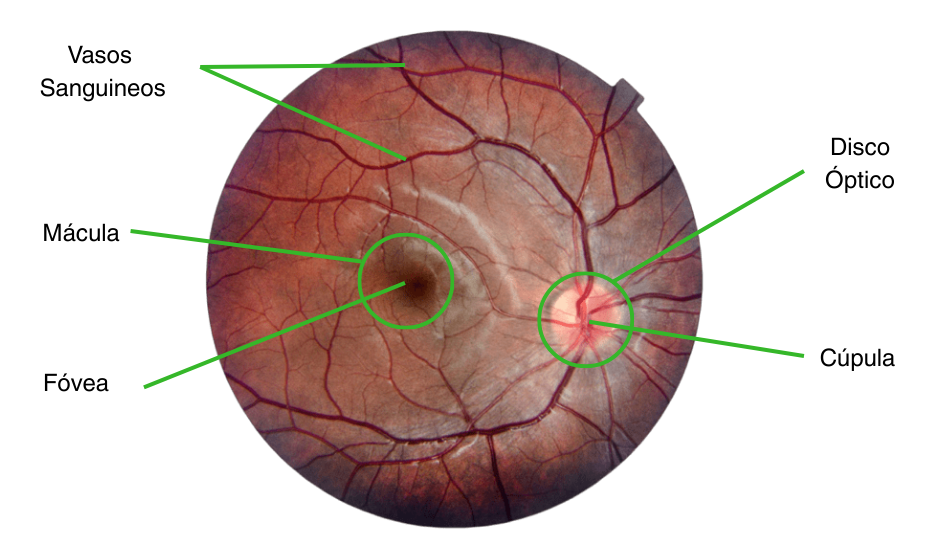
\includegraphics[width=1\textwidth]{imágenes/marco teórico/fundus image.png}
    \caption*{\textit{Fuente: Elaboración propia}}
\end{figure}

En la actualidad podemos encontrar otros tipos de exámenes que pueden ayudar a detectar
la retinopatía diabética. Entre los más conocidos está el examen con lámpara de
hendidura, que permite observar la parte frontal del ojo y la retina; y la tomografía de
coherencia óptica (OCT), que toma secciones transversales de la retina y es útil para
evaluar el grosor y detectar edema macular. Sin embargo, las imágenes del fondo de ojo
son las más utilizadas en la detección de la RD debido a que proporcionan una
visualización directa de la retina, donde se producen los cambios patológicos
característicos, y son relativamente fáciles de interpretar, lo que permite un
diagnóstico rápido. Además, con el avance de la inteligencia artificial, estas imágenes
pueden ser analizadas automáticamente mediante algoritmos de aprendizaje profundo,
permitiendo un tamizaje masivo y eficiente.

\section{RETINOPATÍA DIABÉTICA}

La retinopatía diabética es una complicación ocular de la diabetes que se produce debido
al daño en los vasos sanguíneos de la retina, el tejido sensible a la luz en la parte
posterior del ojo. Este daño es causado principalmente por niveles elevados de glucosa en
la sangre, que pueden obstruir los pequeños vasos sanguíneos que alimentan la retina.
Este daño hace que los vasos sanguíneos se vuelvan más permeables y propensos a filtrar
líquido y sangre en la retina. Además, los vasos sanguíneos pueden hincharse y formar
microaneurismas, que son pequeñas protuberancias en los vasos sanguíneos que pueden
romperse y sangrar.

Esta enfermedad puede tener consecuencias graves para la visión. Una de las
complicaciones más comunes es el sangrado dentro del ojo, que ocurre cuando se forman
vasos sanguíneos anormales que se rompen y liberan sangre en el interior del ojo. Este
sangrado puede hacer que la visión se vuelva borrosa o incluso se pierda completamente si
es muy grande. Otra complicación seria es el desprendimiento de la retina. Los vasos
sanguíneos anormales pueden generar tejido cicatricial que tira de la retina, lo que
puede hacer que se separe de la parte posterior del ojo.

\section{CLASIFICACIÓN DE LA RETINOPATÍA DIABÉTICA EN IMÁGENES DEL FONDO DE OJO}

Los signos microvasculares retinianos clásicos incluyen microaneurismas, hemorragias,
exudados duros, manchas de algodón, dilatación venosa y perlas, así como diversas
anomalías microvasculares intrarretinianas. En las etapas iniciales de la enfermedad,
muchos de estos síntomas no se manifiestan de manera evidente, lo que hace que el
diagnóstico temprano sea más desafiante. Por esta razón, se recomienda que los pacientes
diabéticos se sometan a exámenes regulares de fondo de ojo, incluso si no experimentan
síntomas. La detección temprana es fundamental, ya que permite la intervención antes de
que la enfermedad progrese, lo que brinda una mayor oportunidad para un tratamiento
eficaz, reduce el riesgo de ceguera y atenúa las complicaciones asociadas a la
retinopatía diabética.

La retinopatía diabética se clasifica en dos formas principales: la retinopatía diabética
no proliferativa (RDNP) y la retinopatía diabética proliferativa (RDP), cada una con
características particulares que influyen en el manejo clínico y el pronóstico de la
enfermedad. En la RDNP, los cambios en los vasos sanguíneos retinianos son generalmente
más leves e incluyen microaneurismas, hemorragias y exudados duros. Aunque estos signos
pueden no afectar gravemente la visión en sus primeras etapas, la progresión sin
tratamiento adecuado puede derivar en la forma proliferativa.

El diagnóstico oportuno es crucial, ya que un control adecuado de los niveles de glucosa
en sangre y la detección temprana de la enfermedad pueden retrasar o incluso evitar el
avance hacia formas más graves de retinopatía. Además, estudios han demostrado que los
pacientes que se someten a exámenes regulares de fondo de ojo tienen una mejor tasa de
preservación de la visión a largo plazo \myfootcite{cusick2005associations}.

\begin{figure}[H]
    \centering
    \caption{Etapas de la retinopatía diabética: (a) leve, (b) moderada, (c) severa, (d)
proliferativa}
    \label{fig:etapas-rd}
    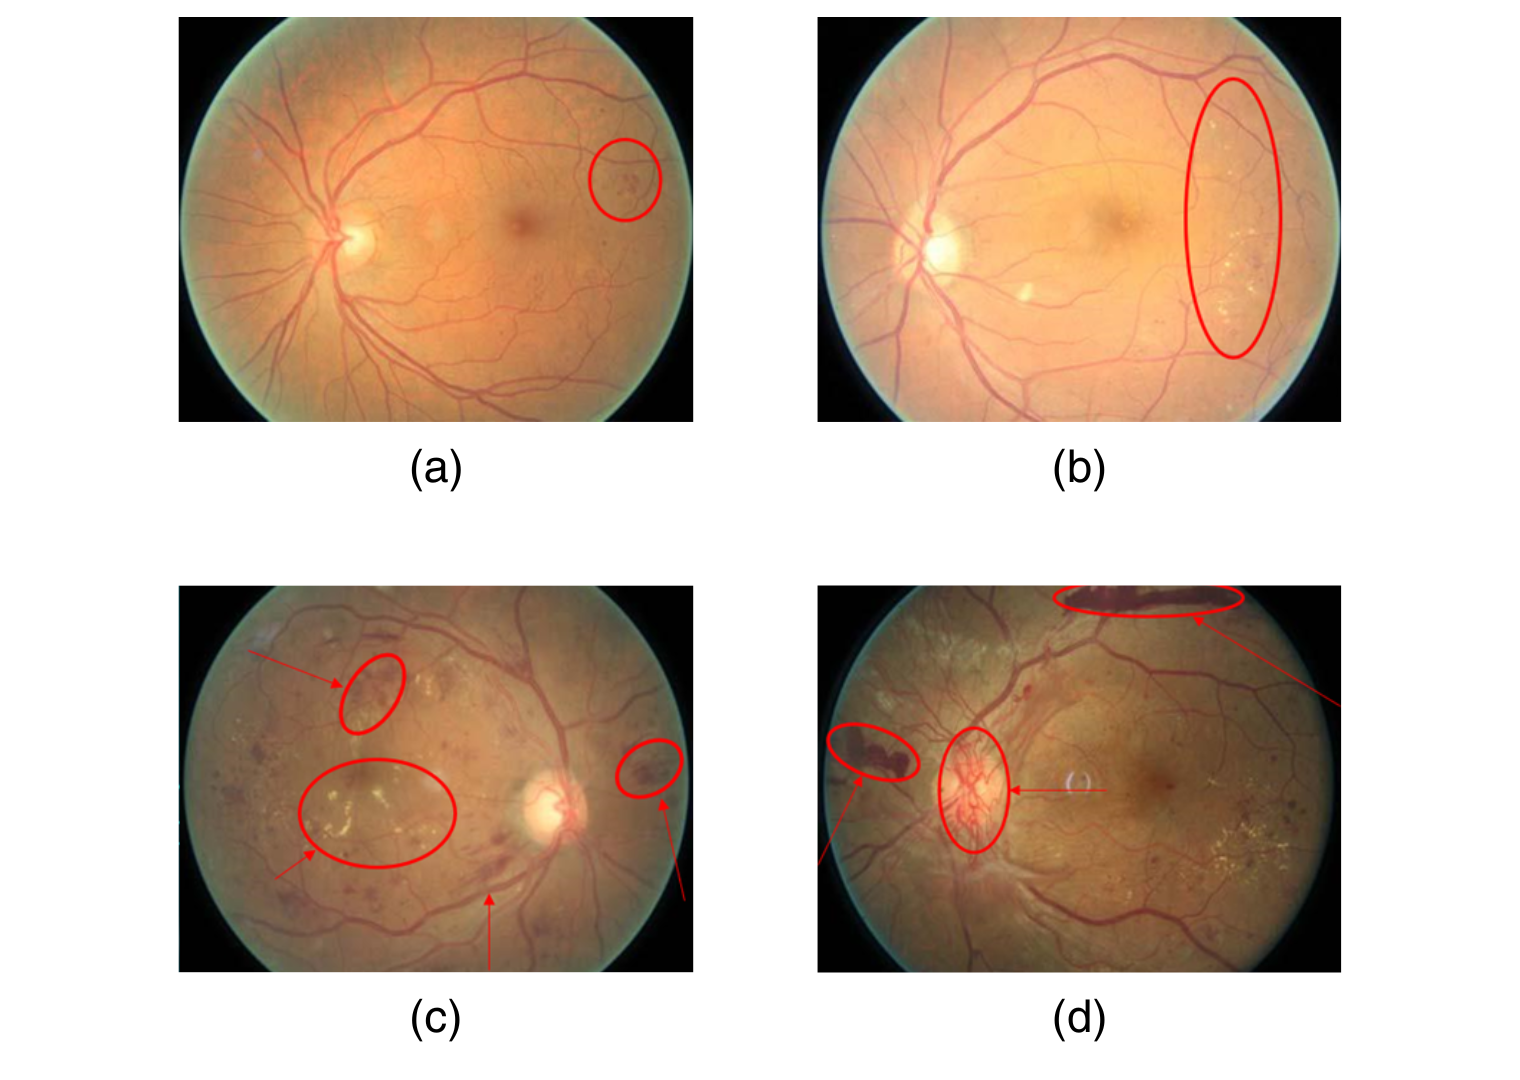
\includegraphics[width=1\textwidth]{imágenes/marco teórico/etapas RD.png}
    \caption*{\textit{Fuente: Adaptado de clasificación clínica estándar de retinopatía
diabética}}
\end{figure}

La retinopatía diabética no proliferativa progresa en varias etapas, como se observa en
la Figura~\ref{fig:etapas-rd}. En la etapa leve (Figura~\ref{fig:etapas-rd}a), los
pequeños vasos sanguíneos de la retina comienzan a debilitarse y desarrollan
microaneurismas, pequeñas protuberancias en las paredes de los vasos, y puede haber una
leve obstrucción que dificulta el suministro de oxígeno y nutrientes a la retina. En la
etapa moderada (Figura~\ref{fig:etapas-rd}b), el deterioro de los vasos sanguíneos se
intensifica, apareciendo más microaneurismas junto con pequeñas hemorragias y exudados,
que son acumulaciones de líquido y proteínas en la retina; también pueden observarse un
engrosamiento de las paredes de los vasos y una disminución en la circulación sanguínea.
En la etapa severa (Figura~\ref{fig:etapas-rd}c), los daños en los vasos sanguíneos son
más significativos, causando una disminución del flujo sanguíneo a la retina, hemorragias
mayores y exudados extensos, así como la formación de tejido fibroso que puede llevar a
la tracción y desprendimiento de la retina. Finalmente, en la etapa proliferativa o
retinopatía diabética proliferativa (RDP) (Figura~\ref{fig:etapas-rd}d), los nuevos vasos
sanguíneos crecen anormalmente en la retina, lo que crea presión en el globo ocular y
puede hacer que la retina se desprenda. Además, la sangre se filtra en el vítreo, lo que
daña el nervio óptico, responsable de transmitir imágenes al cerebro, provocando pérdida
de visión.

\begin{table}[H]
\centering
\renewcommand{\arraystretch}{1.5}
\caption{Etapas de la retinopatía diabética y sus manifestaciones clínicas observables en
oftalmoscopia}
\label{tab:etapas-rd}
\begin{tabularx}{\textwidth}{X X}
\hline
\textbf{Etapa} & \textbf{Hallazgos observables en la oftalmoscopia} \\ \hline
Sin retinopatía aparente & Sin anomalías \\
RD no proliferativa leve & Solo microaneurismas \\
RD no proliferativa moderada & Más microaneurismas \\
RD no proliferativa severa & Hemorragias intrarretinianas mayor a 20 en cada
cuadrante.\newline
Anomalías microvasculares intrarretinianas (en 1 cuadrante) \\
RD proliferativa & Neovascularización\newline
Hemorragia vítrea prerretiniana \\ \hline
\end{tabularx}
\end{table}

\section{INTELIGENCIA ARTIFICIAL}

El estudio de la inteligencia artificial (IA) ha sido una disciplina en constante
evolución durante más de 65 años, impulsada por el esfuerzo conjunto de científicos e
ingenieros. El principio fundamental detrás de la IA es que las máquinas, creadas por el
ser humano, pueden ir más allá de realizar tareas repetitivas o intensivas, desarrollando
una forma de inteligencia que imita o incluso supera ciertas capacidades humanas
\myfootcite{jiang2022quo}.

Uno de los aspectos más destacados de la IA es su capacidad para cambiar el paradigma
tradicional de los algoritmos. En la programación convencional, los datos de entrada son
procesados por un conjunto de reglas predefinidas por el programador, lo que da como
resultado una salida determinada. En contraste, los sistemas de inteligencia artificial
operan mediante un enfoque de aprendizaje automático, donde se proporcionan conjuntos de
datos de entrada y salida, pero el algoritmo debe aprender por sí mismo las reglas y
patrones subyacentes que relacionan ambos conjuntos. Esto permite que el programa sea
capaz de inferir correlaciones entre datos y, con el tiempo, adaptar su comportamiento,
mejorando su precisión y eficiencia sin intervención humana directa.

En el ámbito de la medicina, la inteligencia artificial ha mostrado un crecimiento
impresionante y continúa ganando terreno. Año tras año se incrementa su uso, a medida que
los avances en la ciencia computacional permiten desarrollar tecnologías más sofisticadas
y eficaces. Un ejemplo de ello son los robots quirúrgicos, que realizan procedimientos
con una precisión milimétrica, minimizando riesgos y mejorando los tiempos de
recuperación. Asimismo, se han creado sistemas de IA que analizan grandes cantidades de
datos clínicos para clasificar y diagnosticar enfermedades con una exactitud comparable a
la de los expertos humanos \myfootcite{gulshan2016development}. Además, la IA también se
está utilizando para predecir brotes epidémicos, personalizar tratamientos médicos y
mejorar la gestión de los servicios de salud en general. A medida que la investigación
avanza, es probable que veamos aplicaciones aún más innovadoras de la IA, que no solo
transformarán la manera en que abordamos la medicina, sino que también influirán en una
gran cantidad de otras industrias.

\subsection{APRENDIZAJE AUTOMÁTICO}

El aprendizaje automático (machine learning) es un subcampo de la inteligencia artificial
que ha transformado profundamente la manera en la que interactuamos con la tecnología. Se
refiere a la capacidad de las máquinas de aprender a partir de los datos que se les
proporcionan, sin necesidad de ser programadas de manera explícita para cada tarea
específica. Estos sistemas utilizan algoritmos matemáticos complejos para identificar
patrones dentro de grandes volúmenes de datos, y luego emplean esos patrones para hacer
predicciones o tomar decisiones autónomas.

El proceso de aprendizaje automático comienza con la recopilación de datos, que es
crucial para obtener resultados precisos. La calidad de los datos tiene una influencia
directa sobre el rendimiento del modelo, por lo que es fundamental que los datos sean
representativos, completos y correctos. En muchas ocasiones, los datos deben ser
preprocesados para asegurar que se encuentren en una forma adecuada para ser procesados
por los algoritmos, lo que incluye tareas como la normalización, la eliminación de
valores atípicos o la imputación de datos faltantes.

Existen diversos tipos de algoritmos de aprendizaje automático, entre los cuales destacan
la clasificación, regresión y clustering, y la selección del algoritmo adecuado depende
del tipo de problema que se desee resolver. Una vez que se cuenta con los datos
preparados, se procede a entrenar el modelo ajustando sus parámetros internos de manera
que se minimicen los errores en las predicciones. Durante este proceso, el modelo aprende
a realizar la tarea que se le ha asignado, mejorando su capacidad para generalizar a
datos que no haya visto previamente. Finalmente, el rendimiento del modelo se evalúa
utilizando un conjunto de datos de prueba, lo que permite verificar que el modelo sea
capaz de generalizar bien y no esté simplemente memorizando los datos de entrenamiento.

Dentro del campo del aprendizaje automático, existen diferentes tipos o enfoques según la
estructura de los datos y el tipo de tarea que se desea realizar. Los principales son: el
aprendizaje supervisado, el no supervisado, el semisupervisado y el aprendizaje por
refuerzo. En el aprendizaje supervisado se realiza el entrenamiento utilizando un
conjunto de datos etiquetado, es decir, datos para los cuales ya se conoce la salida
correcta. El objetivo es que el modelo pueda mapear nuevas entradas a sus respectivas
salidas correctas (etiquetas). Los modelos de clasificación y regresión son ejemplos
típicos de aprendizaje supervisado. En clasificación, el objetivo es asignar una etiqueta
a un conjunto de datos (por ejemplo, determinar si una imagen contiene un perro o un
gato), mientras que en regresión el objetivo es predecir un valor continuo (como el
precio de una casa en función de características como su tamaño y ubicación)
\myfootcite{jordan2015machine}.

Por otro lado, en el aprendizaje no supervisado el modelo trabaja con un conjunto de
datos que no tiene etiquetas, y el objetivo es identificar patrones ocultos dentro de los
datos. Por ejemplo, el modelo puede buscar agrupaciones de datos similares (clustering) o
intentar reducir la cantidad de características necesarias para representar los datos
(reducción de dimensionalidad). Este tipo de aprendizaje se utiliza ampliamente en
análisis exploratorio de datos y en tareas como la segmentación de clientes o la
detección de anomalías.

En el enfoque del aprendizaje semisupervisado se combinan elementos del aprendizaje
supervisado y no supervisado. En este caso, el conjunto de datos contiene tanto ejemplos
etiquetados como no etiquetados. Este enfoque es útil cuando etiquetar grandes cantidades
de datos es costoso o impráctico, pero se dispone de un pequeño conjunto de datos
etiquetados para guiar el proceso de aprendizaje. Los algoritmos semisupervisados
intentan aprovechar los datos no etiquetados para mejorar el rendimiento general del
modelo.

Por último, el aprendizaje por refuerzo se basa en el concepto de recompensa y
penalización. En este paradigma, un agente toma decisiones en un entorno y recibe
recompensas o penalizaciones en función de las acciones que realiza. El objetivo es que
el agente aprenda a tomar decisiones que maximicen la recompensa acumulada a largo plazo.
Este enfoque se utiliza en tareas complejas donde las decisiones deben tomarse en
secuencia, como en la robótica, el juego de ajedrez o la conducción autónoma.

\subsection{REDES NEURONALES CONVOLUCIONALES}

En el campo de la visión por computadora, las redes neuronales convolucionales (CNN, por
sus siglas en inglés) y sus posteriores mejoras han representado un hito crucial en el
procesamiento de imágenes. El uso de estas fue popularizado por el trabajo de Yann LeCun
y colaboradores en 1998 \myfootcite{lecun1998gradient}. Antes de la aparición de las CNN,
las redes neuronales artificiales tradicionales tenían limitaciones significativas para
trabajar con datos de más de una dimensión, como es el caso de las imágenes. Las redes
neuronales convencionales están diseñadas para procesar arreglos numéricos
unidimensionales. Estos arreglos no son ideales para procesar imágenes, las cuales, al
ser tratadas por un computador, se representan como matrices bidimensionales de valores
numéricos (en el caso de las imágenes en escala de grises) o tridimensionales (para
imágenes en color).

Para que una red neuronal tradicional pueda procesar imágenes, debe aplanar estas
matrices multidimensionales, convirtiéndolas en un arreglo unidimensional. Este proceso
implica perder la relación espacial entre los píxeles vecinos, lo que resulta en una
pérdida significativa de información contextual, esencial para tareas de clasificación y
detección de patrones. Como resultado, el modelo es menos efectivo al capturar
características importantes que dependen de la estructura espacial de los datos.

Mientras que las redes neuronales convolucionales resuelven este problema al procesar las
imágenes en su formato original de múltiples dimensiones. Una CNN utiliza una operación
denominada convolución, que consiste en aplicar un filtro (o kernel) a lo largo de la
imagen. Este filtro también es un arreglo de varias dimensiones que se desplaza sobre la
imagen, realizando una operación de multiplicación elemento a elemento entre el filtro y
las porciones de la imagen con las que coincide. El filtro "captura" patrones locales,
como bordes, texturas o formas, y extrae información relevante de estas coincidencias. Al
repetir este proceso a través de diferentes áreas de la imagen, se generan mapas de
características que preservan las relaciones espaciales y las características locales de
la imagen. El resultado final es una representación más rica y estructurada de la imagen,
que proporciona una mejor base para tareas de clasificación, segmentación o
reconocimiento de patrones.

Una red neuronal convolucional profunda, o CNN profunda, está compuesta por múltiples
capas organizadas en una estructura jerárquica. Cada capa tiene una función específica
que contribuye al proceso de extracción de características y toma de decisiones.

\begin{figure}[H]
	\centering
	\caption{Estructura general de una Red Neuronal Convolucional}
	\label{fig:cnn-general}
	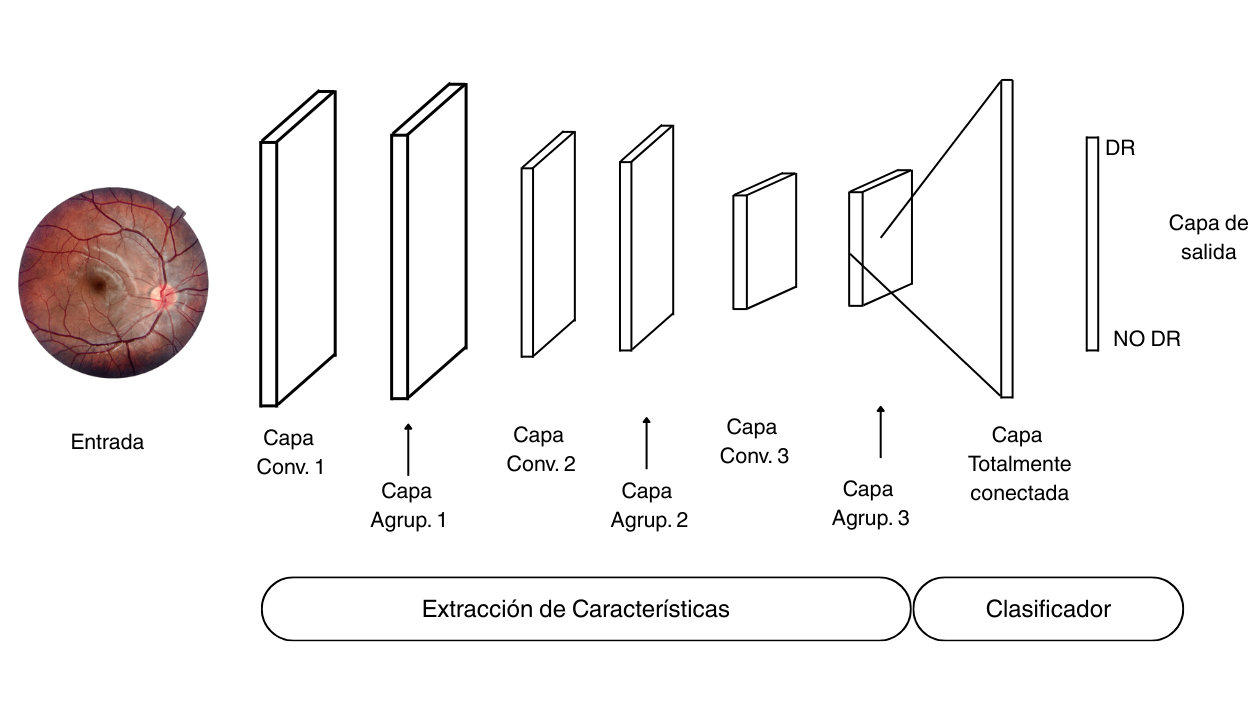
\includegraphics[width=1\textwidth]{imágenes/marco teórico/cnn.png}
	\caption*{\textit{Fuente: Adaptado de arquitecturas CNN estándar}}
\end{figure}

\textbf{Capa convolucional:} Es la primera capa de una red convolucional y su 
componente fundamental: se encarga de extraer la información relevante de la imagen.
Internamente, esta capa está formada por varios filtros de tamaño  $M \times N$
que se deslizan sobre la imagen de entrada hasta recorrerla toda. En cada desplazamiento, 
se calcula el producto punto entre los valores del filtro y los de la región correspondiente
de la imagen. Con estos resultados se construye el mapa de características. Estos mapas revelan
patrones locales como bordes y esquinas, y se utilizan como entrada para capas posteriores, 
que aprenden rasgos más complejos \myfootcite{purwono2022understanding}.

\begin{figure}[H]
	\centering
	\caption{Ejemplo de operación de convolución utilizando un paso de 1 con un
kernel de $3 \times 3$}
	\label{fig:convolution}
	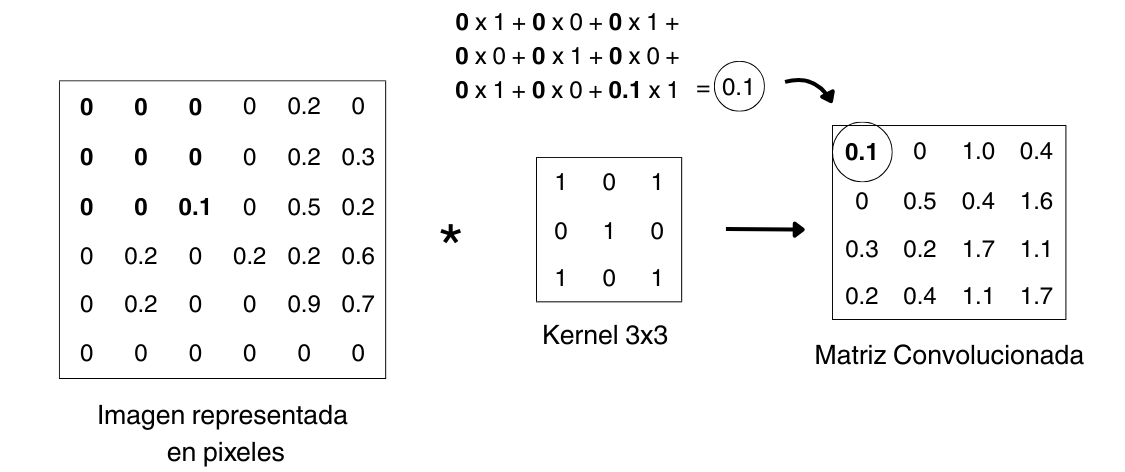
\includegraphics[width=1\textwidth]{imágenes/marco teórico/capa_convolucional.png}
	\caption*{\textit{Fuente: Adaptado de operaciones estándar de CNN}}
\end{figure}

\textbf{Función de activación:} Se aplica una función de activación después de cada
operación de convolución. Esta función ayuda a la red a aprender relaciones no lineales
entre las características de la imagen, lo que hace la red más robusta para identificar
distintos patrones. También ayuda a mitigar el problema de desvanecimiento de gradiente.
Las funciones de activación más comunes incluyen ReLU (Rectified Linear Unit), Sigmoid y
Tanh.

\textbf{Capa de agrupamiento:} La capa de agrupación (también llamada pooling) va después
de una capa de convolución, y su propósito es reducir el tamaño espacial del mapa de
características, es decir, su ancho y alto \myfootcite{akgul2024pooling}. Este proceso
disminuye el costo computacional y ayuda a condensar la información local. Las
operaciones de agrupación se aplican a secciones del mapa de características y producen
una versión reducida que conserva lo más importante. Las variantes más usadas son:

\begin{itemize}
    \item \textbf{Max pooling:} para cada sección, selecciona el valor más alto.
    \item \textbf{Average pooling:} calcula la media de los valores en la sección.
    \item \textbf{Min pooling:} selecciona el valor más bajo en cada sección.
\end{itemize}

\begin{figure}[H]
	\centering
	\caption{Ejemplo de max-pooling con un paso de 2 utilizando un filtro de $2
\times 2$}
	\label{fig:maxpooling}
	
\includegraphics[width=0.9\textwidth]{imágenes/marco
teórico/capa_agrupamiento.png}
	\caption*{\textit{Fuente: Adaptado de operaciones estándar de pooling}}
\end{figure}

\textbf{Capa Multi-Head Attention:} Este tipo de bloques fueron introducidos por primera
vez en la arquitectura de transformers \myfootcite{vaswani2017attention}. En esencia, son
un mecanismo que permite a un modelo de IA enfocarse en diferentes partes de una
secuencia de datos y analizar las partes más determinantes de la misma. Estos bloques se
componen de varias "cabezas de atención", por lo que es posible observar los datos desde
múltiples perspectivas. Cada cabeza de atención trabaja con tres elementos principales: Q
(queries), K (keys) y V (values), que son representaciones diferentes de la misma
información de entrada.

En visión computacional, la atención se ha usado de dos maneras complementarias: como
sustituto completo de las convoluciones en arquitecturas tipo ViT (Vision Transformer)
para procesar secuencias de parches, y como complemento de redes convolucionales,
concatenando o integrando mapas de características de atención con los mapas
convolucionales para incorporar contexto no local. En particular, trabajos que integran
atención con CNNs han mostrado mejoras consistentes en clasificación y detección, incluso
en arquitecturas diseñadas para dispositivos móviles \myfootcite{dosovitskiy2020image}.

\textbf{Capa GaussianNoise:} Este tipo de capas aplican durante el entrenamiento una
perturbación aditiva. En términos generales, cada valor de la activación de la capa
recibe ruido gaussiano aleatorio durante la fase de entrenamiento y la capa queda
inactiva durante la inferencia. Esta acción puede interpretarse como una forma de aumento
estocástico aplicado a las características internas de la red y como un regularizador que
evita el sobreajuste al exponer al modelo a versiones ligeramente corruptas de las
representaciones aprendidas. En redes con backbones preentrenados, las capas añadidas
para clasificación suelen contener muchos parámetros nuevos y son especialmente propensas
a sobreajustarse cuando los datos etiquetados disponibles son limitados. Introducir ruido
gaussiano sobre el mapa de características sirve para forzar a que el clasificador
aprenda patrones robustos y no dependientes de valores exactos de activación, y para
simular variabilidad propia de la adquisición de imágenes (ruido del sensor, diferencias
de iluminación o preprocesado). Estudios empíricos en problemas clínicos y de visión han
mostrado mejoras en métricas de generalización y AUC cuando se usa inyección de ruido
\myfootcite{zur2009noise}.

\textbf{Capa completamente conectada:} La capa completamente conectada (FC) está formada
por pesos, sesgos y neuronas. Actúa como un puente que conecta las neuronas que están
presentes entre las capas ocultas y las capas de salida. Estas capas se colocan solo unas
pocas capas antes de la capa de salida. El mapa de características de la capa anterior se
aplana para crear un único vector de características largo. El vector aplanado se pasa a
otras capas completamente conectadas en las que se realizan muchas operaciones
matemáticas. El proceso de clasificación comienza en esta etapa. La
Figura~\ref{fig:flattening} muestra un ejemplo de proceso de aplanamiento que convierte
las características en una única dimensión.

\begin{figure}[H]
    \centering
    \caption{Proceso de Aplanamiento (Flattening) de un Mapa de Características}
    \label{fig:flattening}
    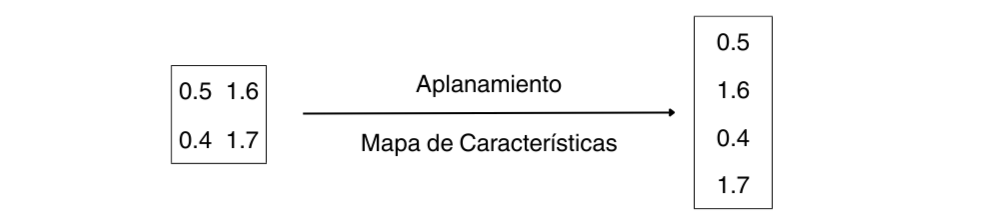
\includegraphics[width=1\textwidth]{imágenes/marco teórico/aplanamiento.png}
    \caption*{\textit{Fuente: Elaboración propia}}
\end{figure}

\subsection{SOBREAJUSTE Y REGULARIZACIÓN}

El sobreajuste (overfitting) es un problema habitual en los modelos de aprendizaje
automático. Ocurre cuando el modelo aprende demasiado los datos de entrenamiento,
incluyendo su ruido y sus valores atípicos, lo que se conoce como "aprendizaje de
memoria". Un aprendizaje de este tipo conduce a un modelo que funciona bien con los datos
de entrenamiento, pero mal con nuevos datos no vistos. Por el contrario, el subajuste
(underfitting) ocurre cuando el modelo es demasiado simple para capturar los patrones
subyacentes en los datos.

\begin{figure}[H]
	\centering
	\caption{Ilustración de subajuste, ajuste adecuado y sobreajuste}
	\label{fig:overfitting}
	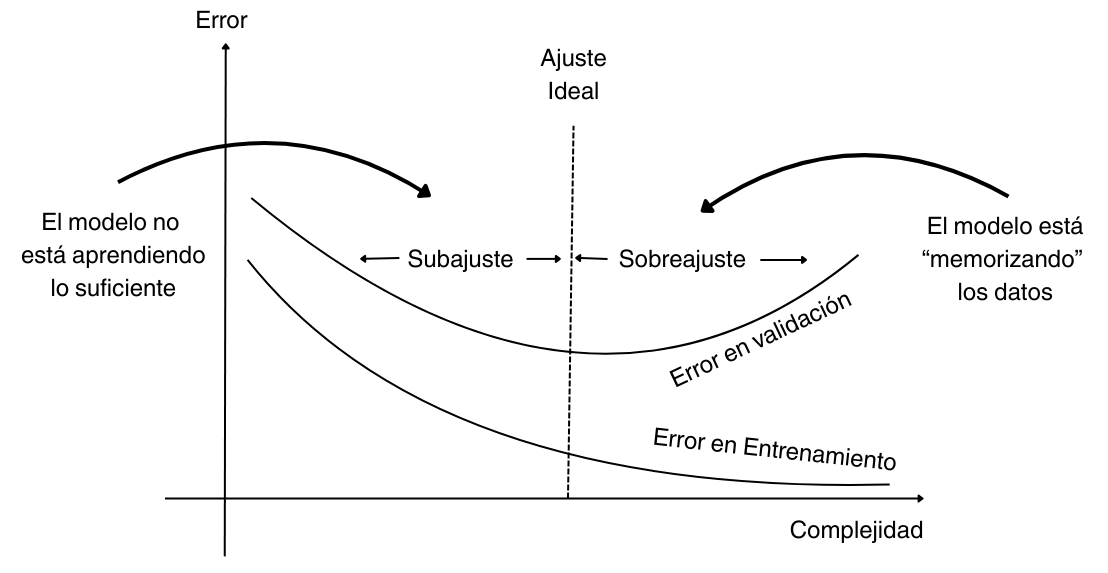
\includegraphics[width=1\textwidth]{imágenes/marco teórico/sobreajuste.png}
	\caption*{\textit{Fuente: Adaptado de conceptos estándar de machine learning}}
\end{figure}

Los modelos de aprendizaje profundo, especialmente las redes neuronales convolucionales
(CNN), son especialmente susceptibles al sobreajuste debido a su alta capacidad y su
habilidad para aprender patrones detallados en datos a gran escala. Existen varias
técnicas de regularización para mitigar el sobreajuste en las CNN. Entre las más comunes
encontramos:

\textbf{Dropout (Abandono):} Esta técnica se basa en desactivar aleatoriamente una
proporción de neuronas durante el entrenamiento, lo que obliga a la red a no depender
excesivamente de neuronas específicas y promueve una representación más robusta de los
datos \myfootcite{garbin2020dropout}. Típicamente, el porcentaje que se desactiva suele
variar entre 0.2 y 0.5. Durante el entrenamiento, las conexiones de las neuronas
desactivadas se eliminan temporalmente, lo que resulta en una red más ligera en cada paso
de entrenamiento. La implementación de esta técnica ha mostrado ser particularmente
efectiva en redes densamente conectadas para mejorar la generalización.

\textbf{Normalización por lotes (Batch Normalization):} El sobreajuste se reduce en
cierta medida normalizando la capa de entrada mediante el ajuste y la escala de las
activaciones. Este enfoque también se utiliza para acelerar y estabilizar el proceso de
entrenamiento al reducir la covarianza interna del modelo.

\textbf{Capas de agrupamiento (Pooling):} Estas capas pueden utilizarse para reducir las
dimensiones espaciales de la imagen de entrada y proporcionar al modelo una forma
abstracta de representación, reduciendo así la posibilidad de sobreajuste al disminuir el
número de parámetros.

\textbf{Parada Anticipada (Early Stopping):} Esta técnica consiste en monitorear el
rendimiento del modelo en un conjunto de validación durante el proceso de entrenamiento y
detenerlo cuando dicho rendimiento deja de mejorar. Así se evita que el modelo se ajuste
demasiado a los datos de entrenamiento y pierda capacidad de generalización. Este método
ha sido probado en distintas investigaciones \myfootcite{brownlee2018gentle}, donde se
demuestra que el early stopping puede reducir el sobreajuste y mejorar la generalización
de las redes neuronales profundas.

\textbf{Inyección de ruido:} Este proceso consiste en añadir ruido a las entradas o a las
salidas de las capas ocultas durante el entrenamiento para hacer más robusto el modelo e
impedir que generalice débilmente.

\textbf{Regularización L1 y L2:} Las técnicas de regularización L1 y L2 consisten en
agregar un término de penalización a la función de pérdida para evitar el sobreajuste.

La regularización L1 (Lasso) añade una penalización proporcional a la suma de los
valores absolutos de los pesos:

\begin{equation}
L_{total} = L_{original} + \lambda \sum_{i} |w_i|
\end{equation}

Esta penalización tiende a llevar los pesos hacia cero, lo que produce modelos dispersos
(\textit{sparse}) y facilita la selección automática de características al eliminar
aquellas menos relevantes.

Por su parte, la regularización L2 (Ridge) añade una penalización proporcional a la
suma de los cuadrados de los pesos:

\begin{equation}
L_{total} = L_{original} + \lambda \sum_{i} w_i^2
\end{equation}

A diferencia de L1, esta técnica reduce la magnitud de los pesos sin llevarlos
exactamente a cero, lo que contribuye a una mayor estabilidad numérica y distribuye
el peso entre características correlacionadas. En ambos casos, $\lambda$ es el hiperparámetro que controla la magnitud de la
penalización. En \myfootcite{kukavcka2017regularization} se presenta una taxonomía
de métodos de regularización en el aprendizaje profundo, destacando la efectividad
de estas técnicas en la mejora de la capacidad de generalización de las redes neuronales.

\textbf{Aumento de datos (Data Augmentation):} Es el proceso de aumentar artificialmente
el tamaño y la diversidad del conjunto de datos de entrenamiento mediante la aplicación
de transformaciones aleatorias, como rotación, escalado, volteo o recorte, a las imágenes
de entrada. Esta técnica es especialmente útil en dominios donde obtener datos
etiquetados es costoso, como en imágenes médicas.

\subsection{APRENDIZAJE POR TRANSFERENCIA}

El aprendizaje por transferencia es un enfoque avanzado dentro del campo del aprendizaje
automático que ha ganado considerable popularidad, especialmente en aplicaciones de
aprendizaje profundo. En este método, un modelo previamente entrenado para realizar una
tarea específica se reutiliza como punto de partida para entrenar un segundo modelo en
una tarea relacionada. Este enfoque es comúnmente utilizado en arquitecturas de redes
neuronales profundas, donde los pesos y parámetros de un modelo previamente entrenado se
transfieren para ser utilizados en un nuevo contexto, lo que permite acelerar el proceso
de entrenamiento y mejorar los resultados en tareas similares.

El aprendizaje por transferencia ofrece múltiples ventajas significativas. Entre ellas
destaca una reducción considerable del tiempo de entrenamiento, ya que al aprovechar
modelos preentrenados que ya han aprendido patrones y características en conjuntos de
datos extensos y generales, se evita entrenar desde cero, lo cual es especialmente
valioso cuando se dispone de datos limitados o se busca reducir costos computacionales
\myfootcite{tan2018survey}. Además, esta técnica permite lograr una mayor precisión y
eficiencia en tareas complejas, como clasificación de imágenes o procesamiento de
lenguaje natural, mediante el ajuste selectivo de capas específicas en lugar de entrenar
toda la red neuronal desde cero \myfootcite{zhuang2020comprehensive}. Por último, el
aprendizaje por transferencia mejora el rendimiento con menos datos, pues al reutilizar
conocimientos adquiridos previamente en conjuntos grandes y diversos, el modelo puede
generalizar mejor incluso con volúmenes reducidos de datos, optimizando así su capacidad
de predicción \myfootcite{weiss2016survey}.

\textbf{Modelo fuente:} Es el modelo previamente entrenado que se selecciona de un
conjunto de modelos candidatos. Este modelo ya ha sido entrenado en un conjunto de datos
grande y general, como ImageNet, y ha aprendido a reconocer patrones y características en
los datos. El modelo fuente proporciona una base sólida que el nuevo modelo puede
aprovechar.

\textbf{Modelo de reutilización:} Una vez que se ha elegido el modelo fuente, este se
utiliza como punto de partida para un nuevo modelo que debe ser entrenado en una tarea
diferente pero relacionada. Dependiendo de los requisitos del problema y de las técnicas
utilizadas, se puede optar por reutilizar todo el modelo o solo ciertas partes, como las
capas de la red que han aprendido características generales (por ejemplo, bordes y
texturas en el caso de imágenes).

\textbf{Ajuste fino (Fine-tuning):} Después de reutilizar el modelo entrenado, es posible
que sea necesario ajustar o afinar ciertas partes del modelo para que se adapte mejor a
los nuevos datos y tareas. Este proceso implica ajustar los pesos del modelo para que se
especialice en las etiquetas de salida del nuevo conjunto de datos, lo cual se logra a
través de una cantidad reducida de entrenamiento adicional.



\section{ARQUITECTURAS DE REDES NEURONALES CONVOLUCIONALES UTILIZADAS}

La retinopatía diabética es una enfermedad ocular compleja y de diagnóstico desafiante,
que requiere una alta precisión en la detección de cambios sutiles en las imágenes del
fondo de ojo. Los modelos preentrenados, especialmente aquellos basados en arquitecturas
profundas de redes neuronales convolucionales (CNN), han demostrado ser eficaces en
tareas de procesamiento de imágenes. Dado que estos modelos han aprendido a identificar
patrones de alto nivel en datos visuales durante su entrenamiento previo, pueden
transferir ese conocimiento a la tarea de identificación de lesiones retinianas, como
microaneurismas, exudados y hemorragias, mejorando la exactitud del diagnóstico.

A continuación se detallan las cuatro arquitecturas de CNN seleccionadas para este
trabajo experimental, elegidas por sus características complementarias en términos de
complejidad, eficiencia computacional y capacidad de generalización.

\subsection{MOBILENETV2}

MobileNetV2 es una red neuronal convolucional optimizada para dispositivos móviles y
aplicaciones con recursos limitados. Fue presentada por Google en 2018 por Mark Sandler,
Andrew Howard, Menglong Zhu y colaboradores \myfootcite{sandler2018mobilenetv2}.
MobileNetV2 está diseñada para ser eficiente tanto en términos de número de parámetros
como en cálculos requeridos, lo que la hace adecuada para dispositivos con recursos
limitados. La principal novedad de MobileNetV2 respecto a la versión anterior
(MobileNetV1) es el uso de bloques residuales invertidos y cuellos de botella lineales,
que permiten que la red mantenga un alto rendimiento mientras reduce la complejidad
computacional.

Al igual que en MobileNetV1, esta red utiliza convoluciones separables en profundidad
(depthwise separable convolutions). Este tipo de convolución separa el filtrado en dos
pasos: una convolución de filtro por canal y una convolución $1 \times 1$ para combinar
los resultados. Este enfoque reduce la cantidad de cálculos y parámetros respecto a las
convoluciones tradicionales.

El corazón de esta arquitectura son los bloques residuales invertidos. En estos, las
características primero se expanden a una dimensión mayor y posteriormente se procesan
mediante una convolución separable en profundidad. Por último, las características se
proyectan de nuevo a una dimensión más baja mediante una convolución de $1 \times 1$.

Otro aspecto único de MobileNetV2 es el uso de cuellos de botella lineales. Esto
significa que después de la expansión de las características, la proyección de vuelta a
un espacio de menor dimensión se realiza sin activaciones no lineales. Este enfoque ayuda
a mantener la representación de características más eficiente, lo que se traduce en una
mayor precisión y velocidad de la red en comparación con las redes tradicionales que usan
activaciones no lineales después de la reducción de dimensiones.

\begin{figure}[H]
	\centering
	\caption{Arquitectura de MobileNetV2 mostrando bloques residuales invertidos}
	\label{fig:mobilenetv2}
	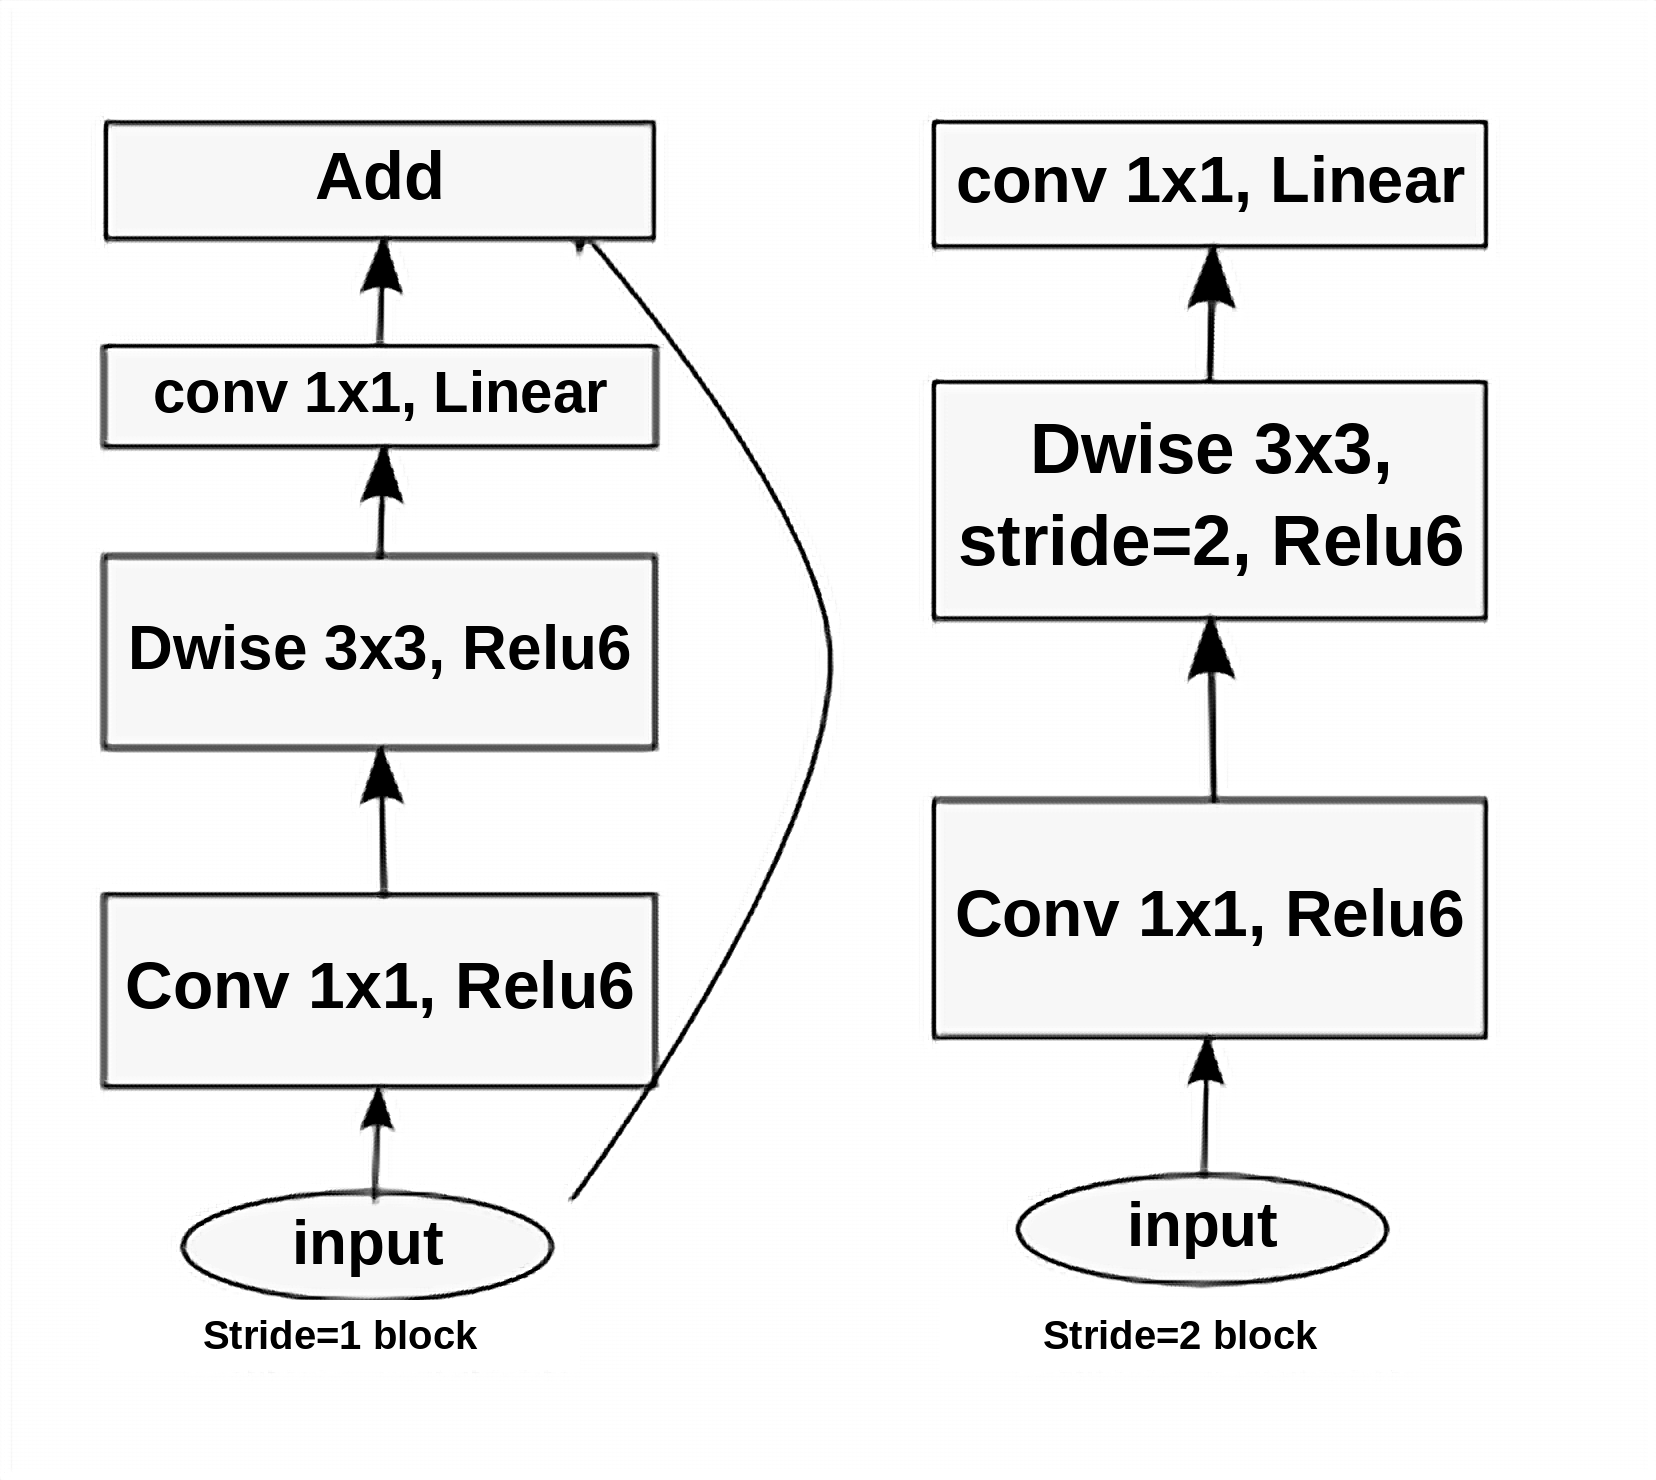
\includegraphics[width=0.8\textwidth]{imágenes/metodología/ArqMobilNetV2.png}
	\caption*{\textit{Fuente: Sandler et al. (2018)}}
\end{figure}

En general, la arquitectura de MobileNetV2 se compone de una serie de bloques residuales
invertidos que incluyen: expansión, la cual es una convolución de $1 \times 1$ que
incrementa la dimensión de características; convolución por profundidad, que es una
convolución separable en profundidad que aplica filtros de tamaño $3 \times 3$; y una
proyección, que es una convolución de $1 \times 1$ que reduce la dimensión de las
características a su tamaño original.

\subsection{RESNET50V2}

ResNet50V2 es una variante mejorada de la arquitectura ResNet (Red Residual) original,
introducida con el objetivo de optimizar el flujo del gradiente durante el entrenamiento
y, en consecuencia, mejorar la capacidad de generalización y rendimiento. Esta versión
fue presentada en el trabajo de Kaiming He, Xiangyu Zhang, Shaoqing Ren y Jian Sun
\myfootcite{he2016identity}.

El núcleo de ResNet, y por ende de ResNet50V2, son los llamados bloques residuales. Estos
bloques incluyen conexiones de salto (skip connections) que permiten que el gradiente
fluya más fácilmente hacia las capas iniciales durante el entrenamiento, mitigando el
problema del desvanecimiento del gradiente en redes muy profundas. En la versión V2, la
principal diferencia respecto a la original (V1) es que se reorganizan las operaciones en
el bloque residual, además de que se incluyen mapeos de identidad mejorados y una mejor
normalización \myfootcite{he2016identity}.

Mientras que en ResNetV1 se utiliza una estructura del tipo convolución seguida de Batch
Normalization y Activación ReLU, en ResNetV2 se antecede la normalización y la activación
antes de la convolución, siguiendo un enfoque de pre-activación. Este cambio en el orden
de las operaciones mejora el flujo de gradientes y facilita el entrenamiento de redes más
profundas.

\begin{figure}[H]
	\centering
	\caption{Arquitectura de ResNet50V2 con bloques residuales mejorados}
	\label{fig:resnet50v2}
	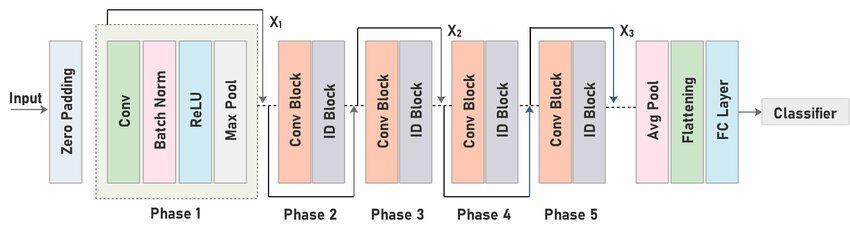
\includegraphics[width=1\textwidth]{imágenes/metodología/arqResNet50v2.jpg}
	\caption*{\textit{Fuente: He et al. (2016)}}
\end{figure}

La arquitectura de esta red está compuesta por 50 capas profundas, organizadas en
distintos bloques residuales con diferentes configuraciones de filtros y tamaños. Cada
bloque residual en ResNet50V2 utiliza una estructura bottleneck, que consiste en tres
capas convolucionales: $1 \times 1$, $3 \times 3$ y $1 \times 1$, lo que permite una
reducción y expansión eficiente de las dimensiones de las características.

\subsection{INCEPTIONV3}

InceptionV3 es una arquitectura de red neuronal convolucional desarrollada para tareas de
clasificación de imágenes, reconocida por su eficiencia y precisión. Es una evolución de
las versiones anteriores de la familia Inception, introducida por Christian Szegedy y
colaboradores de Google, introduciendo mejoras significativas en el procesamiento de
características y la reducción de la complejidad computacional
\myfootcite{szegedy2016rethinking}. La arquitectura busca maximizar la eficiencia del
modelo mediante la optimización de las operaciones convolucionales.

El componente principal de esta red son los módulos Inception. Estos combinan múltiples
tipos de convoluciones y operaciones de pooling en paralelo dentro de una misma capa, lo
que permite a la red capturar información a diferentes escalas y contextos espaciales de
forma simultánea. En esta red, los módulos se optimizan mediante la factorización de
convoluciones más grandes en secuencias de convoluciones más pequeñas y eficientes. Por
ejemplo, una convolución de $5 \times 5$ puede descomponerse en dos convoluciones de $3
\times 3$, reduciendo así el número de parámetros y el costo computacional.

Además, InceptionV3 incorpora capas de reducción de dimensionalidad utilizando
convoluciones $1 \times 1$. Estas capas ayudan a disminuir la dimensionalidad de las
características antes de aplicar convoluciones más costosas, lo que mejora la eficiencia.
También se utiliza la normalización por lotes después de cada convolución, lo que
estabiliza y acelera el entrenamiento al normalizar las activaciones de cada capa.

Otra de las características de la arquitectura de InceptionV3 es el uso de convoluciones
asimétricas para capturar características espaciales de manera más eficiente. Estas
convoluciones permiten que la red mantenga una alta capacidad de representación sin
incrementar significativamente el número de parámetros. Además, para mejorar la
propagación de la información de las etiquetas en las capas inferiores de la red y
mitigar el problema del desvanecimiento del gradiente, InceptionV3 utiliza clasificadores
auxiliares. Estos clasificadores adicionales actúan como regularizadores durante el
entrenamiento, mejorando la convergencia y la precisión del modelo.

\begin{figure}[H]
	\centering
	\caption{Arquitectura de InceptionV3 con módulos Inception paralelos}
	\label{fig:inceptionv3}
	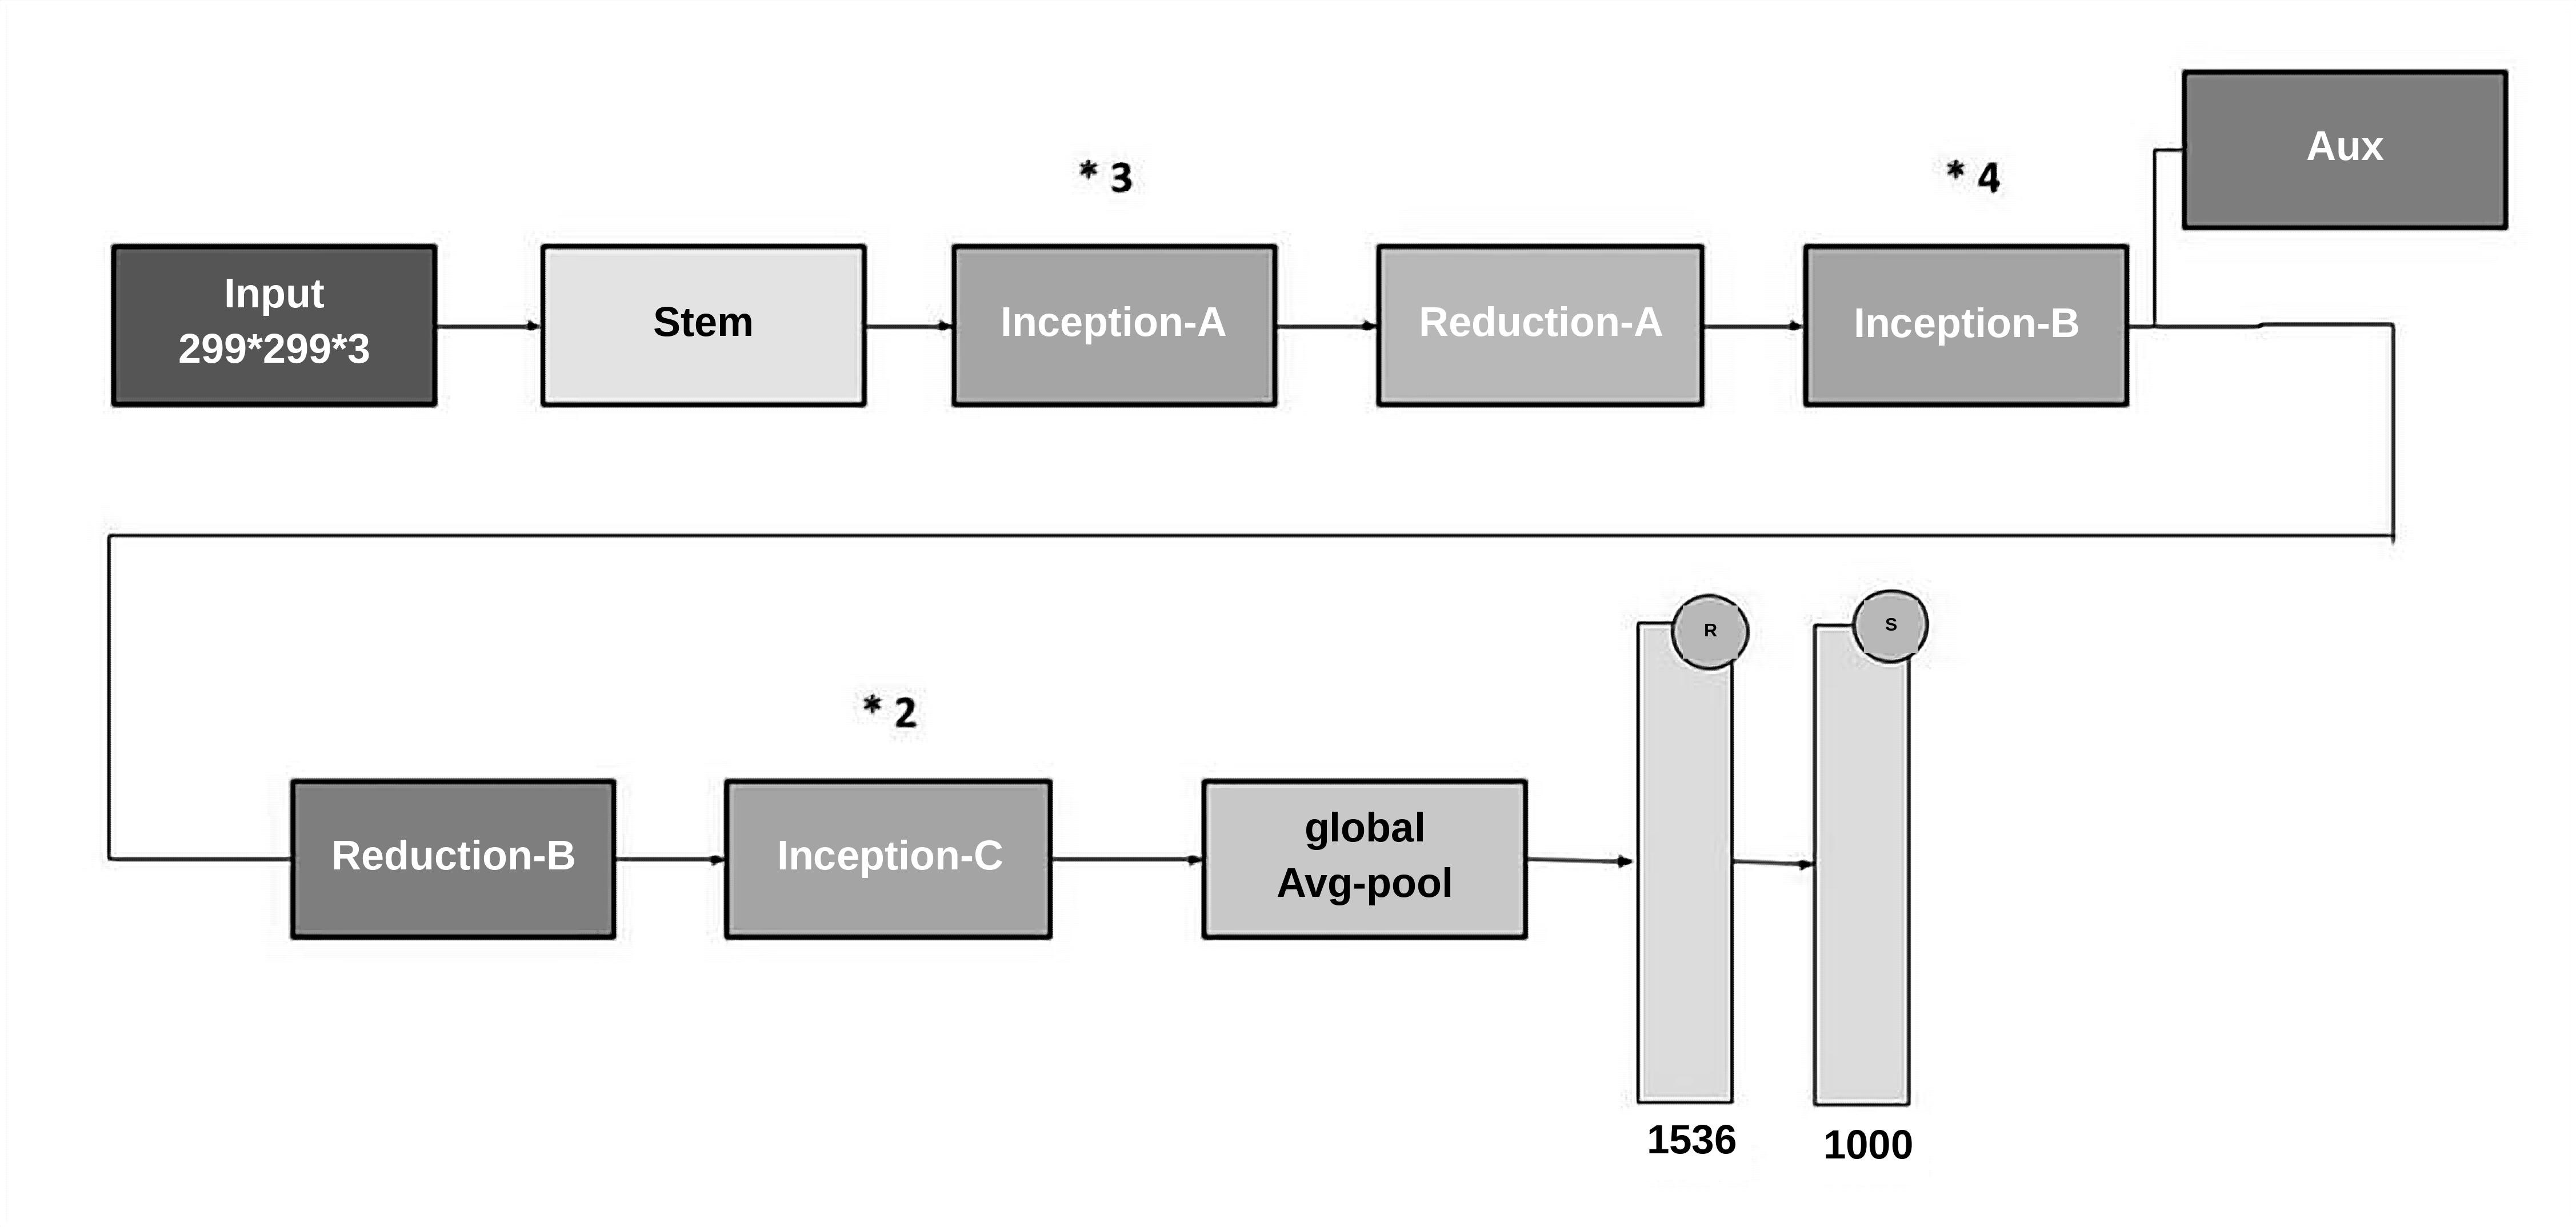
\includegraphics[width=1\textwidth]{imágenes/metodología/Arqinceptionv3.png}
	\caption*{\textit{Fuente: Szegedy et al. (2016)}}
\end{figure}

En general, la arquitectura de InceptionV3 está compuesta por una capa de entrada,
seguida de módulos Inception con factorización de convoluciones y reducción de
dimensionalidad. Por último se aplica una capa de Global Average Pooling seguida de capas
completamente conectadas para la clasificación final.

\subsection{VGG19}

La arquitectura VGG19 pertenece a la familia de redes VGG (Visual Geometry Group) y fue
desarrollada con el objetivo de investigar la relación entre la profundidad de las redes
neuronales y su rendimiento. Esta red convolucional profunda fue introducida por Karen
Simonyan y Andrew Zisserman de la Universidad de Oxford y diseñada específicamente para
tareas de clasificación de imágenes. VGG19 se caracteriza por tener 19 capas en total: 16
de ellas son convolucionales y las 3 restantes son capas completamente conectadas. A
pesar de su complejidad, la arquitectura de VGG19 se distingue por su simplicidad y su
diseño sistemático, en el que se emplean filtros pequeños de $3 \times 3$ píxeles a lo
largo de las capas convolucionales.

La estructura de VGG19 está organizada en bloques secuenciales de capas convolucionales,
seguidos de capas de pooling y finalizando con capas totalmente conectadas. Cada bloque
convolucional consta de entre 2 y 4 capas convolucionales, todas utilizando filtros de
tamaño $3 \times 3$, con un stride de 1 y un padding de 1. Esta configuración permite
mantener el tamaño espacial de las características durante el proceso de extracción, lo
que ayuda a preservar la resolución de las imágenes a medida que se procesan a través de
la red.

Uno de los aspectos clave de VGG19 es su uso de filtros pequeños ($3 \times 3$), lo que
facilita una mayor capacidad de aprendizaje y un control más fino sobre las
características extraídas en cada capa. Además, la red utiliza capas de max pooling para
reducir la dimensionalidad y la complejidad computacional sin perder información
importante.

VGG19 ha sido una de las arquitecturas más influyentes en el campo de la visión por
computadora debido a su rendimiento sobresaliente en tareas de clasificación de imágenes,
como se demostró en la competencia ImageNet. La red también ha sido utilizada como modelo
base en diversos problemas relacionados con el procesamiento de imágenes, adaptándose
fácilmente a tareas como detección de objetos, segmentación y, en el caso de la
retinopatía diabética, clasificación de imágenes médicas.

\begin{figure}[H]
	\centering
	\caption{Arquitectura de VGG19 con bloques convolucionales secuenciales}
	\label{fig:vgg19}
	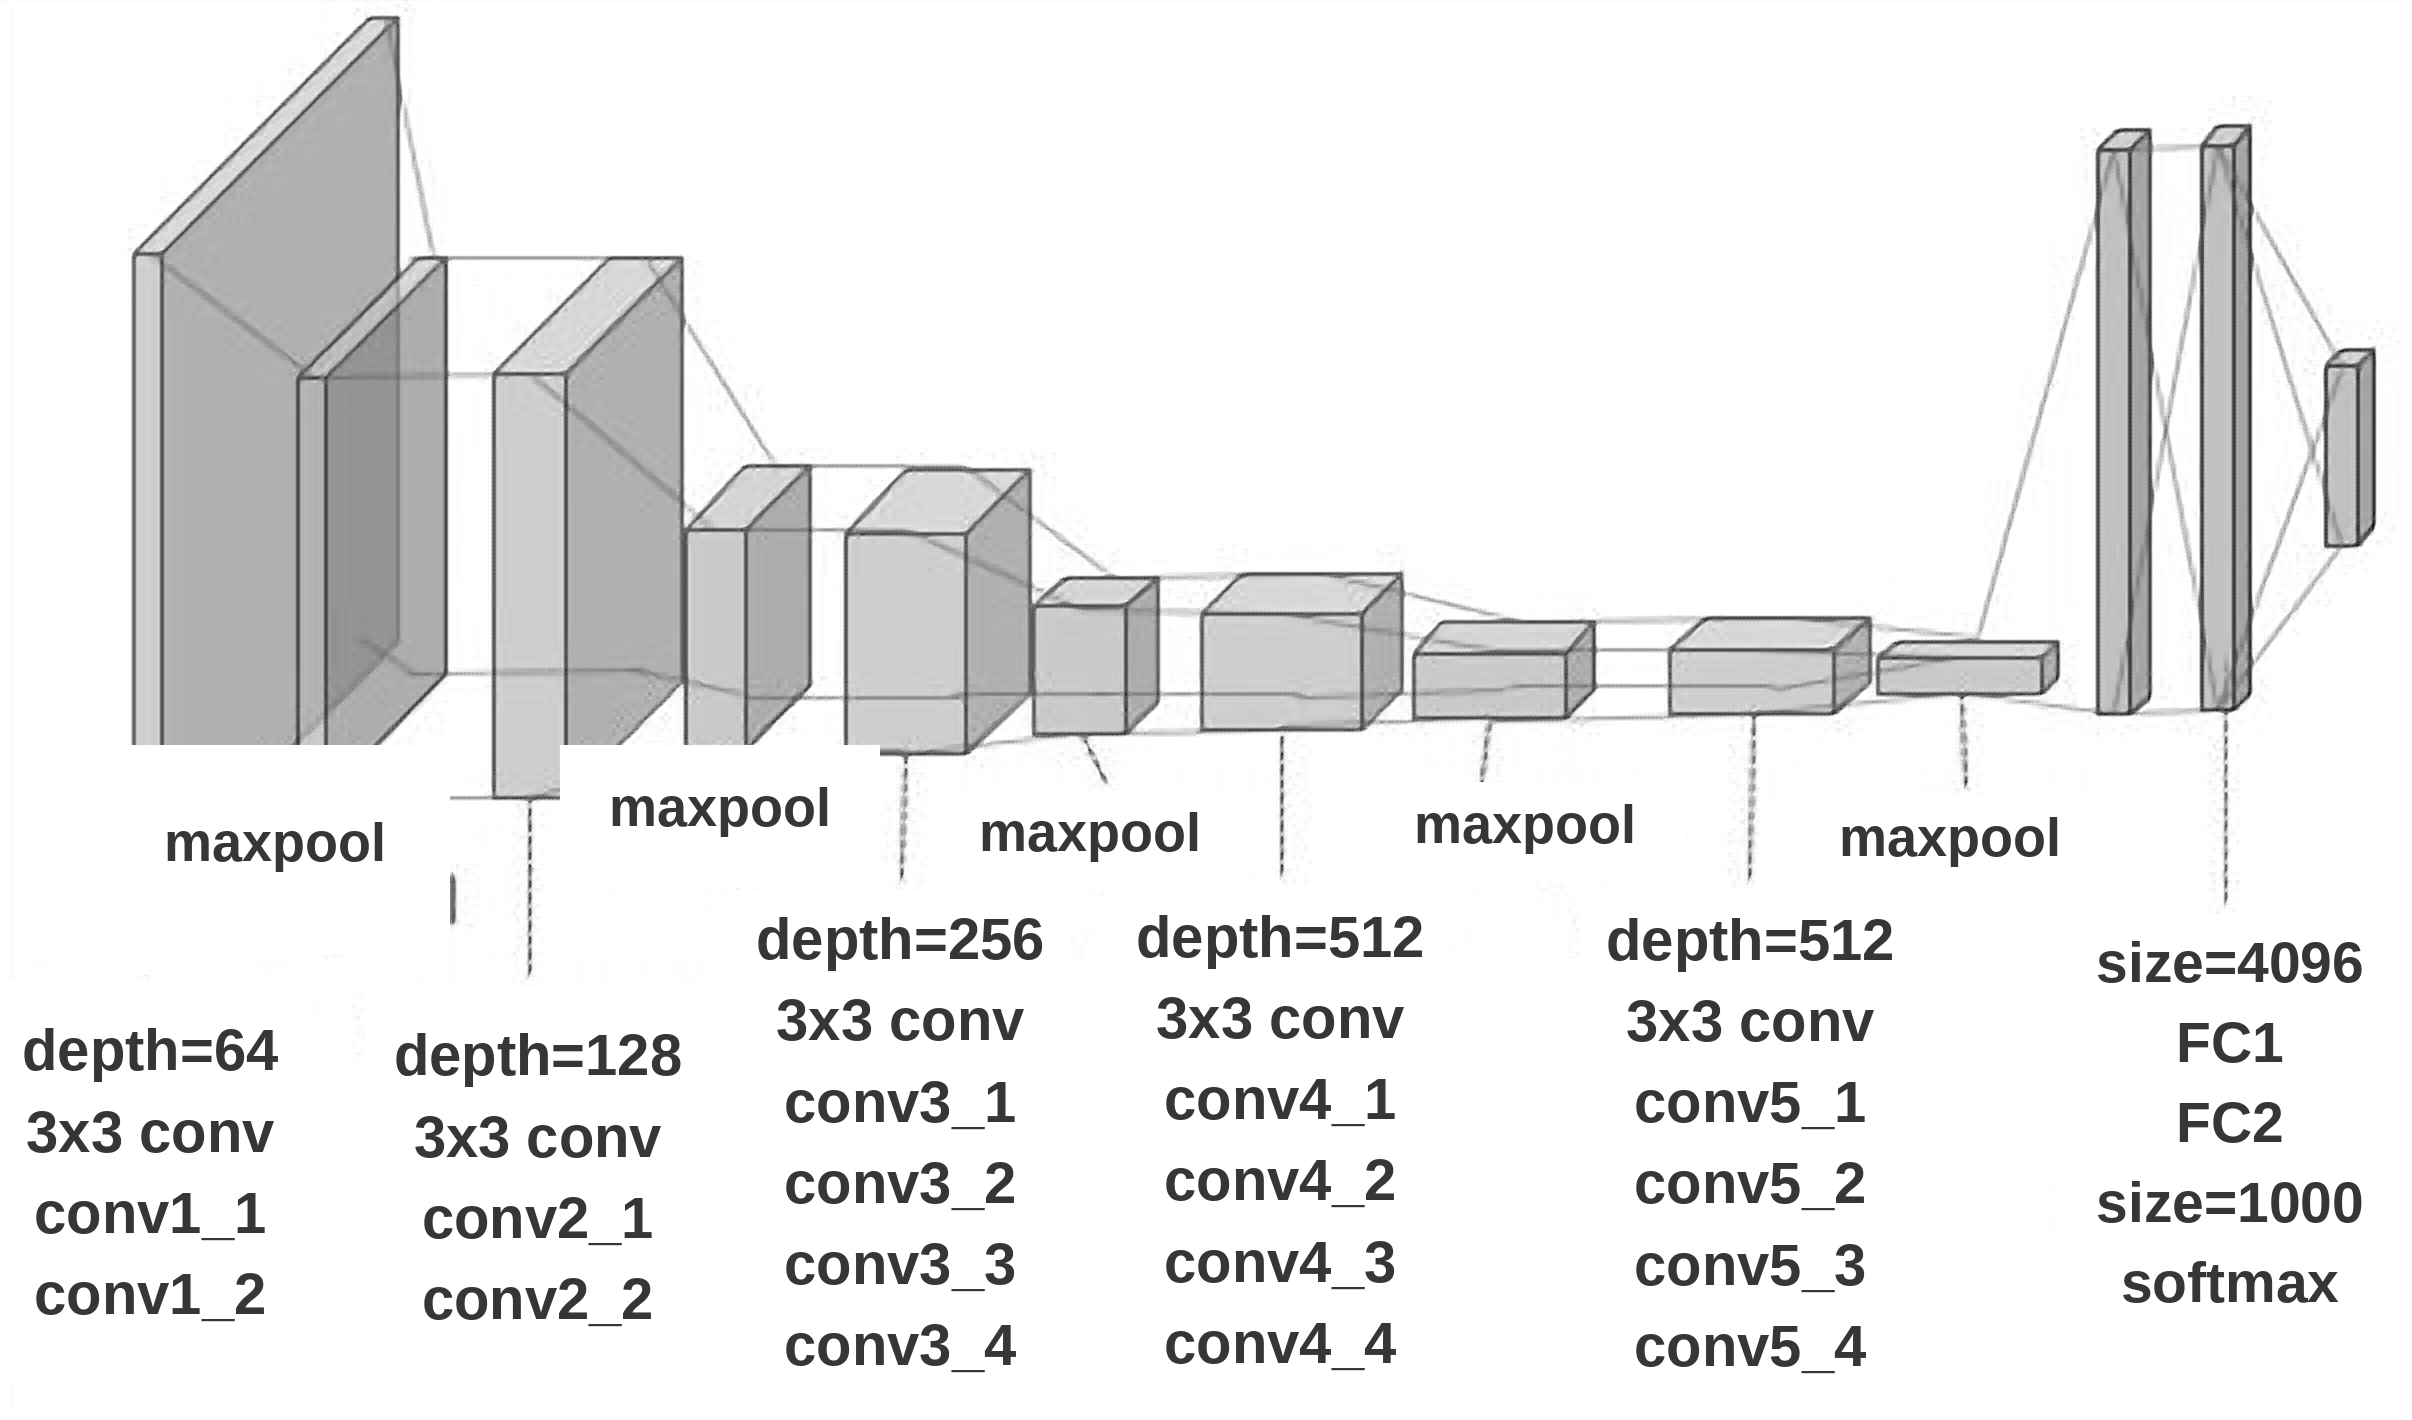
\includegraphics[width=1\textwidth]{imágenes/metodología/arqVgg19.jpg}
	\caption*{\textit{Fuente: Simonyan \& Zisserman (2014)}}
\end{figure}

\subsection{Comparación de arquitecturas}

La Tabla~\ref{tab:comparacion-arquitecturas} presenta una comparación cuantitativa de las
cuatro arquitecturas seleccionadas, considerando aspectos clave para su aplicación en
clasificación de imágenes médicas.

\begin{table}[H]
\centering
\renewcommand{\arraystretch}{1.3}
\caption{Comparación de arquitecturas CNN utilizadas en este trabajo}
\label{tab:comparacion-arquitecturas}
\begin{tabularx}{\textwidth}{l X c c X}
\hline
\textbf{Arquitectura} & \textbf{Características distintivas} & \textbf{Capas} &
\textbf{Parámetros} & \textbf{Ventaja principal} \\ \hline
MobileNetV2 & Bloques residuales invertidos, convoluciones separables & 53 & $\sim$3.5M &
Eficiencia computacional \\
ResNet50V2 & Conexiones residuales con pre-activación & 50 & $\sim$25M & Entrenamiento de
redes profundas \\
InceptionV3 & Módulos Inception paralelos, factorización & 48 & $\sim$24M & Captura
multiescala \\
VGG19 & Arquitectura simple y profunda con filtros 3x3 & 19 & $\sim$144M & Simplicidad
arquitectónica \\ \hline
\end{tabularx}
\end{table}

Cada una de estas arquitecturas aporta características complementarias al estudio
experimental. MobileNetV2 ofrece eficiencia computacional crucial para aplicaciones en
recursos limitados; ResNet50V2 permite entrenar modelos muy profundos sin degradación de
rendimiento; InceptionV3 captura información a múltiples escalas mediante sus módulos
paralelos; y VGG19, a pesar de su mayor cantidad de parámetros, ofrece una arquitectura
simple que ha demostrado efectividad en tareas de clasificación de imágenes médicas.
